\documentclass[11pt,a4paper]{scrartcl}

%\usepackage{scrpage2}
\usepackage{amssymb}
\usepackage{amsmath}
\usepackage{amsthm}
\usepackage[style=authoryear,backend=biber,bibencoding=utf8]{biblatex}
\usepackage{booktabs}
\usepackage{colortbl}
\usepackage{dcolumn}
%\usepackage[flushmargin,ragged]{footmisc}
\usepackage{graphicx}
%\usepackage{ifthen}
%\usepackage{lastpage}
%\usepackage{ngerman}
\usepackage{enumitem}
\usepackage{nag}
%\usepackage{hhline}
%\usepackage{listings}
%\usepackage{xr-hyper}
\usepackage{hyperref}
\usepackage{siunitx}
\usepackage{subfigure}
\usepackage{tabularx}
%\usepackage{xcolor}
\usepackage{xltxtra}
\usepackage{pgf}

%\lstset{basicstyle=\fontfamily{pcr}\selectfont, keywordstyle=\bfseries, language=C++}

\makeatletter
\newcolumntype{d}[1]{>{\DC@{.}{.}{#1}}l<{\DC@end}}
\makeatother

\setkomafont{caption}{\footnotesize}
\setkomafont{captionlabel}{\usekomafont{caption}}

\addbibresource{references.bib}

\newcommand{\I}[1]{_{\text{I}#1}}
\newcommand{\E}[1]{_{\text{E}#1}}
\newcommand{\post}{_{\text{post}}}

\title{Effects of Inhibitory Synaptic Scaling on the Balance of Excitation and 
    Inhibition}
\subtitle{Lab Rotation Project Report}
\author{Jan Gosmann}
\makeatletter
\hypersetup{
  pdftitle={\@title},
  pdfauthor={\@author},
  pdfsubject={},
  pdfkeywords={}
}
\makeatother

\begin{document}
\maketitle

\begin{abstract}
    \footnotesize
    A balance of excitatory and inhibitory inputs is commonly found in cortical 
    neurons. \Textcite{Vogels:2011wr} proposed a model to reach this balanced 
    state by plasticity of inhibitory synapses. In this project I investigated 
    the effect of different decay terms in the learning rule. Using a continuous 
    exponential decay of inhibitory weights a balanced state can be reached 
    while maintaining a neuron's stimulus tuning. Moreover, I explored the 
    effect of additional excitatory plasticity.
\end{abstract}

\section{Introduction}
In many studies \parencite[e.g.][]{Okun:2008db, Froemke:2007fo, Wehr:2003hq, 
    delaRocha:ua} a balance of excitatory and inhibitory input to cortical 
neurons was found. A global balance of the input currents ensures the network 
stability. In addition, excitation and inhibition are coupled in time as well as
co-tuned for different stimulus features. This lets one assume that an 
excitatory input is accompanied by a corresponding inhibitory input 
(fig.~\ref{fig:ff_inhibition}) leading to a more detailed, local balance.

\begin{figure}
    \centering
    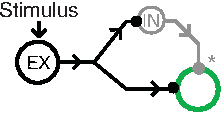
\includegraphics{figures/ff_inhibition}
    \caption{Schematic view of feedforward inhibition where excitation leads to 
        a corresponding inhibition through an indirect pathway. Figure from 
        \textcite{Vogels:2011wr}.}
    \label{fig:ff_inhibition}
\end{figure}

\Textcite{Vogels:2011wr} proposed a mechanism based on plasticity of the 
inhibitory synapses to explain how the balanced state can be reached. Besides 
providing analytical results for the model behavior, they did simulations with 
an integrate-and-fire neuron model. In these a spike-timing-dependent plasticity 
(STDP) learning rule was applied to the inhibitory synaptic weights.  In 
addition to this increase in synaptic weights for nearby pre- and postsynaptic 
spikes a depression of the weights was done for every presynaptic spike.  The 
change of inhibitory synaptic weights $\Delta w\I{}$ can in summary be expressed 
as
\begin{equation}
    \Delta w\I{} = \eta\I{} (\text{pre} \times \text{post} - \rho_0 \times 
    \text{pre})
\end{equation}
with the learning rate $\eta\I{}$, a target firing rate $\rho_0$ and the pre- and 
postsynaptic firing rates $\text{pre}$ and $\text{post}$.

In a lab rotation I analyzed the effects of different modified learning rules 
after reproducing a part of the results of \textcite{Vogels:2011wr}. Also, as 
the excitatory weights were fixed in the original model, I looked at the 
influence of adding spike-timing-dependent learning to these, too.

The report is organized as follows: First, the methods used will be introduced 
in section~\ref{sec:methods}, which is followed by the results and a discussion 
in sections~\ref{sec:results} and \ref{sec:discussion}. Finally, a conclusion 
will be given in section~\ref{sec:conclusion}.

\section{Methods} \label{sec:methods}
All simulations were implemented using the 
Brian\footnote{\url{http://briansimulator.org/}} Python package providing 
a spiking neural network simulator. The model consisted out of a single 
integrate-and-fire neuron receiving input from \num{800} excitatory and 
\num{200} inhibitory synapses. Both types of synapses were divided into eight 
equally sized groups with \num{100} excitatory and \num{25} inhibitory synapses.  
For each group a temporally modulated random rate signal was generated as 
described in the supplementary online material of \textcite{Vogels:2011wr}.  An 
autocorrelation time constant of $\tau_s = \SI{50}{\milli\second}$ was used as 
long as not stated otherwise. From these signals Poisson spike trains with 
a refractory time of \SI{5}{\milli\second} were generated for each synapse.

The effect of incoming spikes at the synapses was modelled as a conductance 
change of the postsynaptic neuron. Excitatory and inhibitory synapses were 
treated separately. I tuned the initial excitatory synaptic weights 
$\mathbf{w}\E{}(\SI{0}{\second})$ to a preferred signal and set the initial 
inhibitory synaptic weights to $w\I{,i}(\SI{0}{\second}) 
= \SI{35}{\pico\siemens}$.

To implement the STDP learning rule synaptic traces $x\I{,i}$, $x\E{,j}$ and 
$x\post$ were assigned to each input spike train $i$, $j$, and the postsynaptic 
neuron.  They increase for every spike by \num{1} and follow an exponential 
decay:
\begin{equation}
    \tau_{\text{STDP}} \frac{dx}{dt} = -x \label{eqn:syntrace}
\end{equation}
Using the synaptic traces the weight $w\I{,i}$ of the $i$-th inhibitory synapse 
will be updated for every postsynaptic spike according to
\begin{equation}
    w\I{,i} \rightarrow w\I{,i} + \eta\I{} \bar g\I{} x\I{,i} \text{.}
\end{equation}
For every presynaptic spike an update was done according to one of the following 
rules:
\begin{align}
    w\I{,i} &\rightarrow w\I{,i} + \eta\I{} \bar g\I{} (x\post - 2 \rho_0 
\tau_{\text{STDP}}) \label{eqn:lr-orig} \tag{\citeauthor{Vogels:2011wr}} \\
    w\I{,i} &\rightarrow w\I{,i} + \eta\I{} \bar g\I{} x\post \label{eqn:lr-no-decay} 
\tag{no decay} \\
    w\I{,i} &\rightarrow w\I{,i} + \eta\I{} \bar g\I{} x\post \qquad\text{(with 
    exponentially decaying weights)} \label{eqn:lr-exp-decay} \tag{exponential 
    decay} \\
    w\I{,i} &\rightarrow w\I{,i} + \eta\I{} \bar g\I{} (x\post - \beta w\I{,i}) 
\label{eqn:lr-weight-dep} \tag{spike related decay}
\end{align}
The rule given in the first equation corresponds to the original learning rule 
from \textcite{Vogels:2011wr}. The \ref{eqn:lr-no-decay} learning rule 
eliminates any decrease in the inhibitory weights. The same equation was coupled 
with an exponential decay of the weights given by
\begin{equation}
    \tau_w \frac{dw\I{,i}}{dt} = -\eta\I{} w\I{,i}
\end{equation}
to obtain the \ref{eqn:lr-exp-decay} learning rule.
Finally, the \ref{eqn:lr-weight-dep} learning rule is conceptually similar to 
the exponentially decaying weights as the decrease depends on the size of the 
weight. However, it is not a steady weight decay, but occurs only for 
presynaptic spikes.

I analyzed the response properties of the trained neuron for training with 
\ref{eqn:lr-orig} and the \ref{eqn:lr-exp-decay} learning rule by calculating 
the squared cross-correlation coefficients between the PSTH and each input 
signal. This I did for two different filter time constants $\tau_s 
= \SI{50}{\milli\second}$ and $\tau_s = \SI{300}{\milli\second}$ controlling the 
duration of autocorrelations in the input signal.

While I kept the excitatory weights constant in the first set of simulations
, I performed a second set of simulations to look at the influence of plasticity 
of the excitatory synapses. The corresponding excitatory synaptic weights were 
updated according to:
\begin{align}
    w\E{,i} &\rightarrow w\E{,i} + \eta\E{} \bar g\E{} x\post \quad\text{for 
    presynaptic spikes} \\
    w\E{,i} &\rightarrow w\E{,i} + \eta\E{} \bar g\E{} x\E{,i} \quad\text{for 
    postsynaptic spikes}
\end{align}
To prevent an unbounded increase in synaptic weights the excitatory synaptic 
weights were normalized in each time step. I tried the multiplicative and 
additive $L^2$ norms:
\begin{align}
    w\E{,i} &\rightarrow 
\frac{\|\mathbf{w}\E{}(\SI{0}{\second})\|_2}{\|\mathbf{w}\E{}\|_2} \cdot w\E{,i} 
\tag{multiplicative $L^2$} \\
    w\E{,i} &\rightarrow w\E{,i} + \|\mathbf{w}\E{}(\SI{0}{\second})\|_2 
- \|\mathbf{w}\E{}\|_2 \tag{additive $L^2$}
\end{align}

\section{Results} \label{sec:results}
The change of the neuron's firing rate and selected synaptic weights are shown 
in figure~\ref{fig:rates_weights}. Using the \ref{eqn:lr-orig} learning rule 
I could reproduce their result. The synaptic weights increase until the firing 
rate is reduced to roughly $\rho_0 = \SI{5}{\hertz}$.  The weights of synapses 
not corresponding to the preferred stimulus overshoot in the beginning and then 
decrease again.

This decrease is blocked using the \ref{eqn:lr-no-decay} learning rule as no 
means to decrease too high inhibitory weights are provided. This results in 
a firing rate close to \SI{0}{Hz}.

The \ref{eqn:lr-orig} learning is not the only way to decrease too large 
weights. Other means for that are demonstrated with the \ref{eqn:lr-exp-decay} 
and \ref{eqn:lr-weight-dep} learning rules. In both cases I could obtain a low 
firing rate larger than zero. Note that the variance of the firing rate is 
higher for the continuous exponential weight decay. During a period of no spikes 
the weights will decrease and lead to a transient high firing rate in the next 
period of spikes.  This variance is decreased by coupling the decrease of 
weights to presynaptic spikes as in the \ref{eqn:lr-orig} and 
\ref{eqn:lr-weight-dep} learning rule.

\begin{figure}
    \centering
    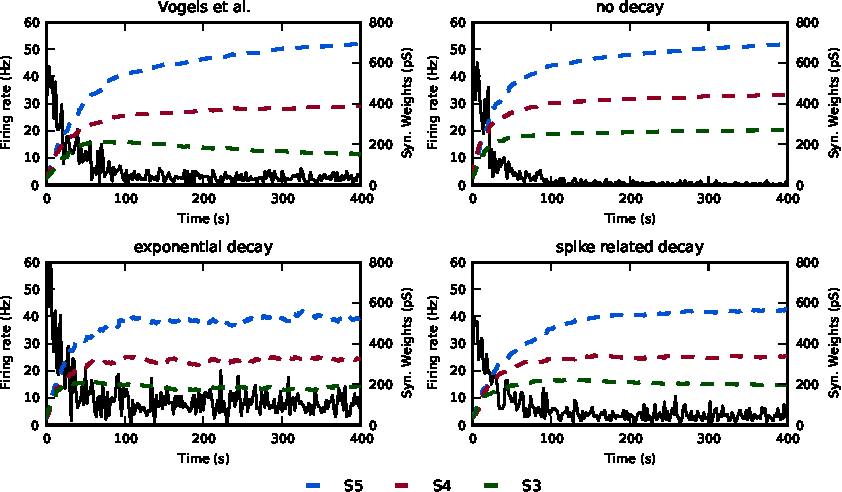
\includegraphics{figures/rates_weights}
    \caption{Firing rate over time for the different learning rules is shown by 
        the solid line. It was determined as the average of \SI{2}{\second} 
        windows. The dashed lines show the average weights of the inhibitory 
        synapses corresponding to certain signals.} \label{fig:rates_weights}
\end{figure}

Figure~\ref{fig:tuning} shows that the tuning of the inhibitory synaptic weights 
matches the excitatory weights after training and thus a local 
inhibition-excitation balance is obtained. In case of the \ref{eqn:lr-no-decay} 
learning rule the sum of some inhibitory weights becomes larger than the sum of 
excitatory weights leading to the near zero firing rate. With the other learning 
rules these weights would be decreased again until a balanced state with 
a certain firing rate is reached.

\begin{figure}
    \centering
    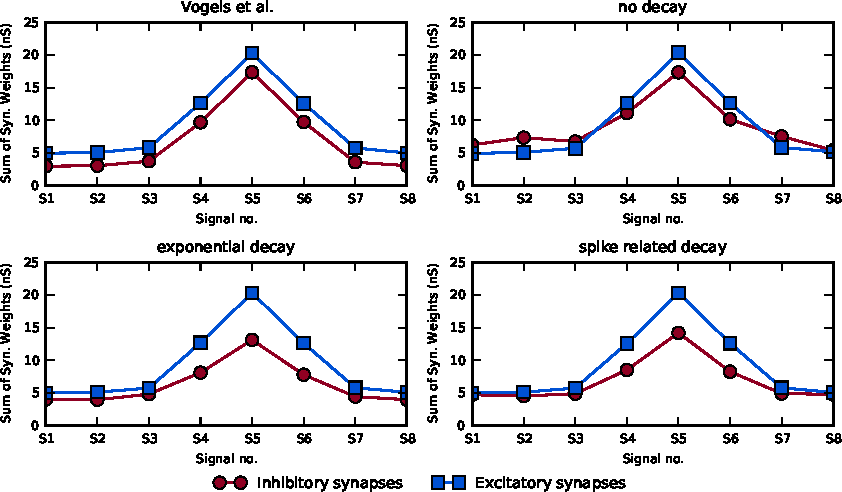
\includegraphics{figures/tuning}
    \caption{Summed weights of synapses associated with a certain signal for 
        different learning rules. These plots show the state after 
        \SI{400}{\second} of learning in simulation time.} \label{fig:tuning}
\end{figure}

Apart from the \ref{eqn:lr-no-decay} learning rule, which leads always to 
a firing rate near zero, the other learning rules provide a parameter allowing 
to control the postsynaptic firing rate after learning. This relationship is 
depicted in figure~\ref{fig:rates}.

\begin{figure}
    \centering
    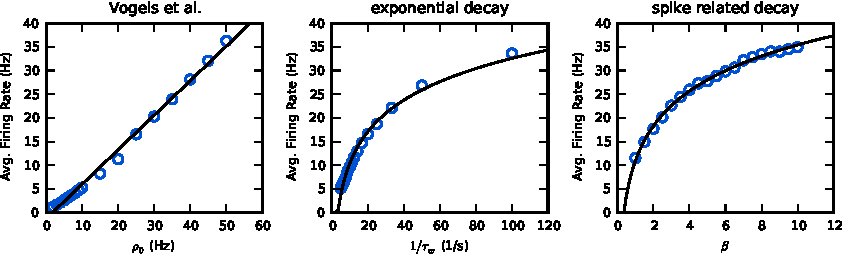
\includegraphics{figures/rates}
    \caption{Firing rates for the different learning rules after learning in 
        dependence of the corresponding parameter. The solid lines are 
        regressions on the data points. In case of the \ref{eqn:lr-orig} 
        learning rule it is linear, in all other cases it is logarithmic.  The 
        firing rates were calculated as the average of a \SI{50}{\second} time 
        window after \SI{50}{\second} of initial learning with $\eta\I{} 
        = 0.01$.} \label{fig:rates}
\end{figure}

The trained neuron's response properties depend on the learning rule used and 
the ``slowness'' of the input signal. In case of the \ref{eqn:lr-orig} learning 
a rule a longer filter time constant $\tau_s$ leads to flatter correlations 
(fig.~\ref{fig:correlations}).
Using the \ref{eqn:lr-exp-decay} learning rule the peak for the preferred signal 
gets much more pronounced because in contrast to the \ref{eqn:lr-orig} learning 
rule the weights are continuously decaying. This means that after a period of no 
input spikes one gets a temporarily increased firing rate of the neuron. This 
effect is even more pronounced for slower signals (larger $\tau_s$) as the 
intervals of no spikes are longer. Therefore, the correlations increase for the 
\ref{eqn:lr-exp-decay} learning rule with larger $\tau_s$ in opposite to the 
\ref{eqn:lr-orig} learning rule.

\begin{figure}
    \centering
    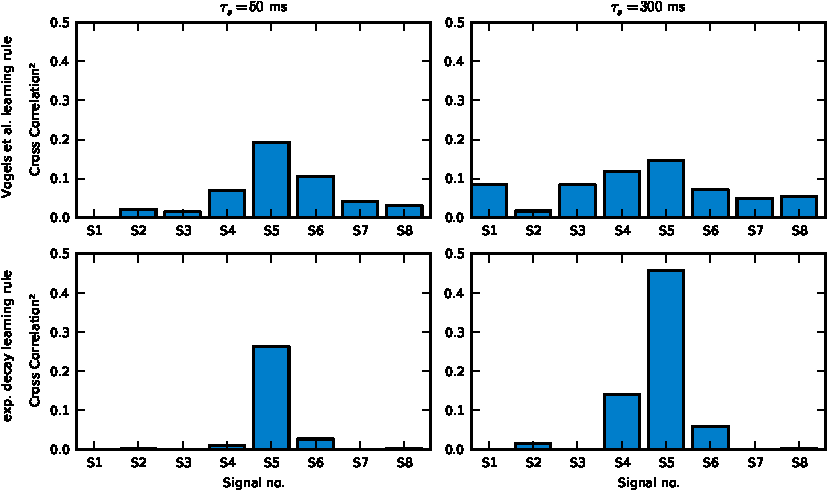
\includegraphics{figures/correlations}
    \caption{Squared cross-correlation coefficients between each input signal 
        and the PSTH. In the top row the synapses were trained with the 
        \ref{eqn:lr-orig} learning rule, while in the bottom row synapses were 
        trained with the \ref{eqn:lr-exp-decay} learning rule. The columns 
        represent different values of the filter time constant $\tau_s$. The 
        PSTH was calculated from \num{500} trials with a stimulus lengths of 
        $400 \tau_s$ after a training period of \SI{400}{\second}.}
    \label{fig:correlations}
\end{figure}

Plastic excitatory synapses with multiplicative normalization in addition to the 
inhibitory plasticity lead easily to oscillations of the synaptic weights 
(fig.~\ref{fig:exc-stdp-mult-l2-main}).  These oscillations are not completely 
regular and their amplitude increases with increasing learning rate ratio 
$\frac{\eta\E{}}{\eta\I{}}$. For a ratio $\frac{\eta\E{}}{\eta\I{}} < 1$ these 
oscillations become damped and the synaptic weights seem to converge to a single 
value with some variation around that value over time. Despite the oscillations 
the target firing rate is maintained.

With the \ref{eqn:lr-exp-decay} learning rule this oscillatory behavior becomes 
less regular and pronounced, but the weights seem not to converge completely for 
$\frac{\eta\E{}}{\eta\I{}} \geq 1$.

The usage of the additive normalization (fig.~\ref{fig:exc-stdp-add-l2}) has the 
effect that the excitatory synaptic weights for preferred stimulus largely 
increase while all other excitatory weights decrease to zero. The inhibition 
follows correspondingly.

\begin{figure}
    \centering
    \subfigure[\ref{eqn:lr-orig} learning 
    rule]{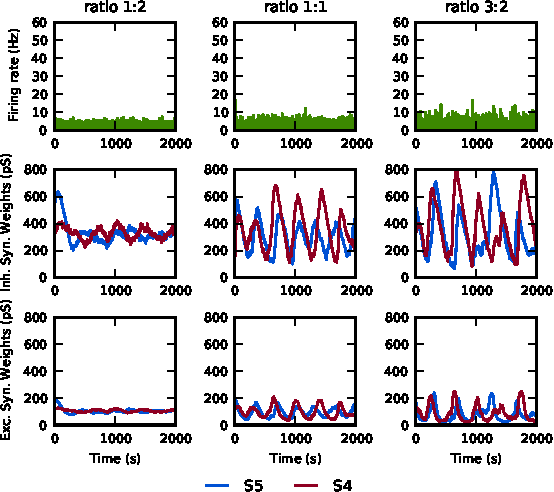
\includegraphics[scale=0.75]{figures/exc-stdp-mult-l2}\label{fig:exc-stdp-mult-l2}}
    \hspace*{2mm}
    \subfigure[\ref{eqn:lr-exp-decay} learning 
    rule]{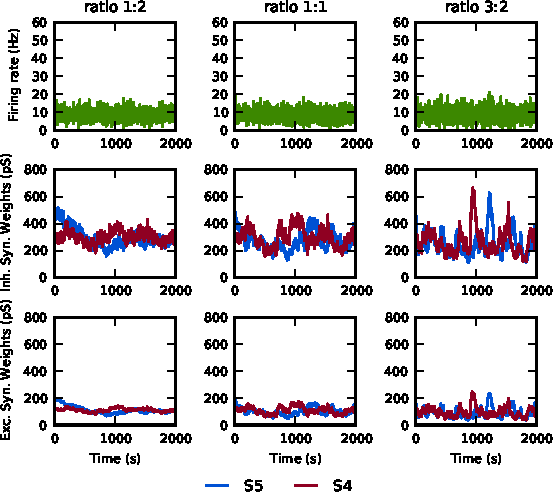
\includegraphics[scale=0.75]{figures/exc-stdp-exp-decay-mult-l2}\label{fig:exc-stdp-exp-decay-mult-l2}}
    \caption{Evolution of firing rate (top row) and synaptic weights for 
        different learning rate ratios $\frac{\eta\E{}}{\eta\I{}}$ in the 
        columns using the \subref{fig:exc-stdp-mult-l2} \ref{eqn:lr-orig} or 
        \subref{fig:exc-stdp-exp-decay-mult-l2} \ref{eqn:lr-exp-decay} learning 
        rule and multiplicative $L^2$ normalization.  The middle row shows the 
        average inhibitory synaptic weights corresponding to two different 
        preferred signals; the bottom row shows the corresponding average 
        excitatory synaptic weights.  An inhibitory learning rate of $\eta\I{} 
        = 0.005$ was used.}
    \label{fig:exc-stdp-mult-l2-main}
\end{figure}
%\begin{figure}
    %\centering
    %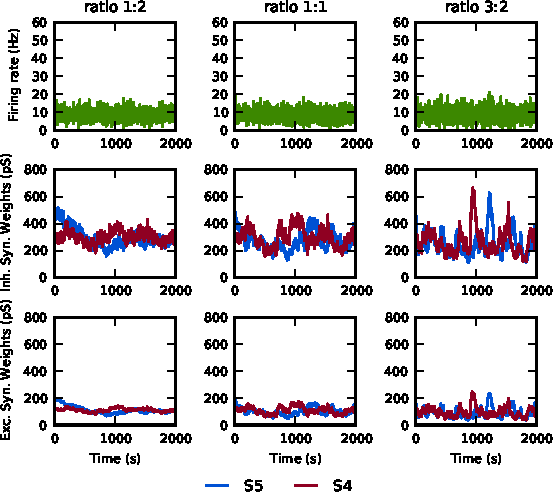
\includegraphics[scale=0.9]{figures/exc-stdp-exp-decay-mult-l2}
    %\caption{Evolution of firing rate (top row) and synaptic weights for 
        %different learning rate ratios $\frac{\eta\E{}}{\eta\I{}}$ in the 
        %columns using the \ref{eqn:lr-exp-decay} learning rule and 
        %multiplicative $L^2$ normalization.  The middle row shows the average 
        %inhibitory synaptic weights corresponding to two different preferred 
        %signals; the bottom row shows the corresponding average excitatory 
        %synaptic weights. An inhibitory learning rate of $\eta\I{} = 0.005$ was 
        %used.}
    %\label{fig:exc-stdp-exp-decay-mult-l2}
%\end{figure}
\begin{figure}
    \centering
    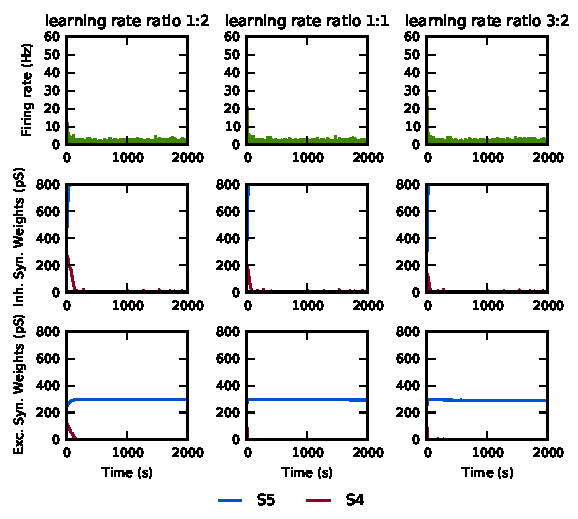
\includegraphics[scale=0.9]{figures/exc-stdp-add-l2}
    \caption{Evolution of firing rate (top row) and synaptic weights using the 
        \ref{eqn:lr-orig} learning rule and additive $L^2$ normalization.  The 
        middle row shows the average inhibitory synaptic weights corresponding 
        to two different preferred signals; the bottom row shows the 
        corresponding average excitatory synaptic weights. A learning rate of 
        $\eta\I{} = \eta\E{} = 0.005$ was used.}
    \label{fig:exc-stdp-add-l2}
\end{figure}

\section{Discussion} \label{sec:discussion}
I could show in this lab rotation project that different learning rules can be 
used to reach a balanced state of excitation and inhibition. To obtain 
a non-zero firing rate it is important to have some mechanism for decreasing too 
large inhibitory weights. Although, different methods yielded a low and 
adjustable firing rate the exact response properties of the neuron to stimuli 
can differ considerable.

With the original \ref{eqn:lr-orig} learning rule the neuron is likely to 
respond in the same way to all stimuli. However, this behavior is not very 
useful as a neuron firing with a constant rate has a limited capability to 
transmit information.  In contrast to that, using the \ref{eqn:lr-exp-decay} 
learning rule the neuron's response is much more correlated with the preferred 
signal than with the other signals.  Nevertheless, the inhibitory and excitatory 
input to the neuron is balanced.

Adding excitatory plasticity with multiplicative normalization can lead to 
oscillations in the synaptic weights.  To prevent this the excitatory synapses 
have to learn at a slower rate. However, all excitatory synaptic weights 
converge then to the same value.  Thus, the neuron loses it's tuning for the 
preferred stimulus and cannot differentiate between the stimuli anymore.

The neuron will keep its tuning to the preferred stimulus when using an additive 
normalization. However, as all other excitatory synaptic weights decrease to 
zero the input from other stimuli could be left out in the first place.

\section{Conclusion} \label{sec:conclusion}
By varying the learning rules of inhibitory plasticity a number of interesting 
response behaviors can be obtained easily. However, this is not as easy with 
added excitatory plasticity. Maybe a more thorough parameter search has to be 
done to find parameters which allow convergence to a balanced state, but also 
keep response properties of the neuron.

Moreover, a mathematical analysis of the influence of excitatory plasticity 
might be useful as it is hard to tell from the simulations where bifurcations 
occur and where the system changes from oscillatory to converging behavior.

\newpage
\appendix
\section{Tabular Description of Model}
Tabular description of the neuron model following \textcite{Nordlie:2009gy}.

\newcommand{\tblsec}[3]{\multicolumn{#1}{l}{\color{white}\cellcolor{black}%
        \makebox[0pt]{\textsf{#2}}\hspace{0.5\linewidth}%
        \makebox[0pt][c]{\textsf{#3}}} \\ \addlinespace}

{
\centering\footnotesize
\begin{tabularx}{\linewidth}{@{}lX@{}} \\
    \tblsec{2}{A}{Model Summary}
    Populations & Single neuron \\
    Topology & --- \\
    Connectivity & --- \\
    Neuron model & Leaky integrate-and-fire, fixed voltage threshold, fixed 
    absolute refractory time \\
    Synapse model & Conductance based inputs (exponentially decaying PSC) \\
    Plasticity & Inhibitory plasticity, excitatory plasticity in some 
    simulations \\
    Input & Poisson spike trains to excitatory and inhibitory synapses \\
    Measurements & Firing rate in \SI{2}{\second} time windows, synaptic 
    weights\\
    \addlinespace \bottomrule
\end{tabularx}

\begin{tabularx}{\linewidth}{@{}llX@{}} \\
    \tblsec{3}{B}{Populations}
    Name & Elements & Size \\
    \cmidrule(r){1-1} \cmidrule(lr){2-2} \cmidrule(l){3-3} \addlinespace
    P & Iaf neuron & Single neuron \\
    \addlinespace \bottomrule
\end{tabularx}

\begin{tabularx}{\linewidth}{@{}lX@{}} \\
    \tblsec{2}{C}{Neuron Model}
    Name & Iaf neuron \\
    Type & Leaky integrate-and-fire, exponential conductance based input 
    synapses \\ \addlinespace
    Subthreshold dynamics & $\tau \frac{dV}{dt} = (V_{\text{rest}} - V) 
    + \frac{1}{g_{\text{leak}}} (g\E{} (V\E{} - V) + g\I{} (V\I{} - V))$ \\ 
    \addlinespace
    Spiking & If $V(t - dt) < \Theta\ \wedge\ V(t) \geq \Theta$:
    \begin{enumerate}[nosep,topsep=0pt,parsep=0pt,partopsep=0pt,itemsep=0pt]
        \item Set $t^{*} = t$.
        \item Emit spike with time-stamp $t^{*}$.
        \item Reset $V(t) = V_{\text{rest}}$.
    \end{enumerate} \\[-\normalbaselineskip]
    \addlinespace \bottomrule
\end{tabularx}

\begin{tabularx}{\linewidth}{@{}lX@{}} \\
    \tblsec{2}{D}{Synapse Model}
    Excitatory & $\tau\E{} \frac{dg\E{}}{dt} = -g\E{} + w\E{,j}(t) \delta(t 
    - t\E{,j}^{*})$ \\ \addlinespace
    Inhibitory & $\tau\I{} \frac{dg\I{}}{dt} = -g\I{} + w\I{,i}(t) \delta(t 
    - t\I{,i}^{*})$ \\
    \addlinespace \bottomrule
\end{tabularx}

\begin{tabularx}{\linewidth}{@{}lX@{}} \\
    \tblsec{2}{E1}{Inhibitory Plasticity Model}
    Name & Inhibitory Spike Time Dependent Plasticity (iSTDP) \\
    Type & Symmetric iSTDP \\
    Acts on & Inhibititory synapses \\ \addlinespace
    Synaptic traces & $\tau_{\text{STDP}} \frac{dx\I{,i}}{dt} = -x\I{,i} 
    + \delta(t - t\I{,i}^{*}),\quad \tau_{\text{STDP}} \frac{dx\post}{dt} = -x\post 
    + \delta(t - t^{*})$ \\ \addlinespace
    Learning rule & For every postsynaptic spike $w\I{,i} \rightarrow w\I{,i} 
+ \eta\I{} \bar g\I{} x\I{,i}$ \newline
For every presynaptic spike of the $i$-th spike train one of 
\begin{itemize}[nosep]
    \item \ref{eqn:lr-orig}: $w\I{,i} \rightarrow w\I{,i} + \eta\I{} \bar g\I{} 
    (x\post - 2 \rho_0 \tau_{\text{STDP}})$
    \item \ref{eqn:lr-no-decay}: $w\I{,i} \rightarrow w\I{,i} + \eta\I{} \bar 
    g\I{} x\post$
    \item \ref{eqn:lr-exp-decay}: $w\I{,i} \rightarrow w\I{,i} + \eta\I{} \bar 
    g\I{} x\post \quad\text{with}\quad \tau_w \frac{dw\I{,i}}{dt} = -\eta\I{} 
    w\I{,i}$
    \item \ref{eqn:lr-weight-dep}: $w\I{,i} \rightarrow w\I{,i} - \eta\I{} \bar 
    g\I{} (x\post - \beta w\I{,i})$
    \end{itemize}\\[-\normalbaselineskip]
    \addlinespace \bottomrule
\end{tabularx}

\begin{tabularx}{\linewidth}{@{}lX@{}} \\
    \tblsec{2}{E2}{Excitatory Plasticity Model (used in some simulations)}
    Name & Excitatory Spike Time Dependent Plasticity (eSTDP) \\
    Type & Symmetric eSTDP \\
    Acts on & Excitatory synapses \\ \addlinespace
    Synaptic traces & $\tau_{\text{STDP}} \frac{dx\E{,i}}{dt} = -x\E{,i} 
    + \delta(t - t\E{,i}^{*}),\quad \tau_{\text{STDP}} \frac{dx\post}{dt} = -x\post 
    + \delta(t - t^{*})$ \\ \addlinespace
    Learning rule & For every postsynaptic spike $w\E{,i} \rightarrow w\E{,i} 
+ \eta\E{} \bar g\E{} x\E{,i}$ \newline
For every presynaptic spike of $j$-th input spike train $w\E{,i} \rightarrow 
w\E{,i} + \eta\E{} \bar g\E{} x\post$ \\
    Normalization & In every time step one of
\begin{itemize}[nosep]
    \item multiplicative $L^2$: $w\E{,i} \rightarrow 
    \frac{\|\mathbf{w}\E{}(\SI{0}{\second})\|_2}{\|\mathbf{w}\E{}\|_2} \cdot 
    w\E{,i}$
    \item additive $L^2$: $w\E{,i} \rightarrow w\E{,i} 
    + \|\mathbf{w}\E{}(\SI{0}{\second})\|_2 - \|\mathbf{w}\E{}\|_2$
\end{itemize}\\[-\normalbaselineskip]
    \addlinespace \bottomrule
\end{tabularx}

\begin{tabularx}{\linewidth}{@{}lX@{}} \\
    \tblsec{2}{F}{Input}
    Type & Description \\
    \cmidrule(r){1-1} \cmidrule(l){2-2} \addlinespace
    Poisson spike trains & Rate modulated Poisson spike trains with absolute 
    refractory time. Rate modulation was done by $N_S$ random signals with an 
    autocorrelation time constant $\tau_s$.  Spike train groups of 
    $\frac{N_{\text{E}}}{N_S}$ excitatory and $\frac{N_{\text{I}}}{N_S}$ 
    inhibitory synapses were fed by spike trains modulated with the same signal.  
    \\
    \addlinespace \bottomrule
\end{tabularx}
}

\section{Simulation Parameter Summary}
Tabular summary of simulation parameters following \textcite{Kunkel:2011gj}. If 
multiple values are given, the first value was used where not otherwise noted.

{
\centering\footnotesize
\input{params}
}

\printbibliography

\end{document}
